\documentclass[11pt]{beamer}
\usetheme{CambridgeUS}
\usepackage[utf8]{inputenc}
\usepackage{amsmath}
\usepackage{amsfonts}
\usepackage{amssymb}
\usepackage{graphicx}

\author{Nico Fröhlich}
\title{Advanced CPU design and optimization}

\setbeamercovered{transparent} 
\setbeamertemplate{navigation symbols}{} 
\institute{Troblecodings} 
\subject{IT}

\begin{document}

\begin{frame}
    \titlepage
\end{frame}

\begin{frame}{Quellen und weiterführende Inhalte}
    \begin{itemize}
        \item Intel® 64 and IA-32 Architectures Software Developer’s Manual
        \item Software Optimization Guide for AMD64 Processors
        \item Intel® 64 and IA-32 Architectures Optimization Reference Manual
        \item Chandler Carruth, Matt Godbolt, Andrei Alexandrescu ...
        \item Mike Acton
    \end{itemize}
\end{frame}

\begin{frame}{Einführung}
Das was alle CPUs gemeinsam haben:
    \begin{itemize}
        \item Clock (Oszillator)
        \item Fetch-Decode Cycle
        \item Instruction Counter
    \end{itemize}
\end{frame}

\begin{frame}{Fetch - Decode - Execute Cycle}
\begin{figure}[hbtp]
\centering
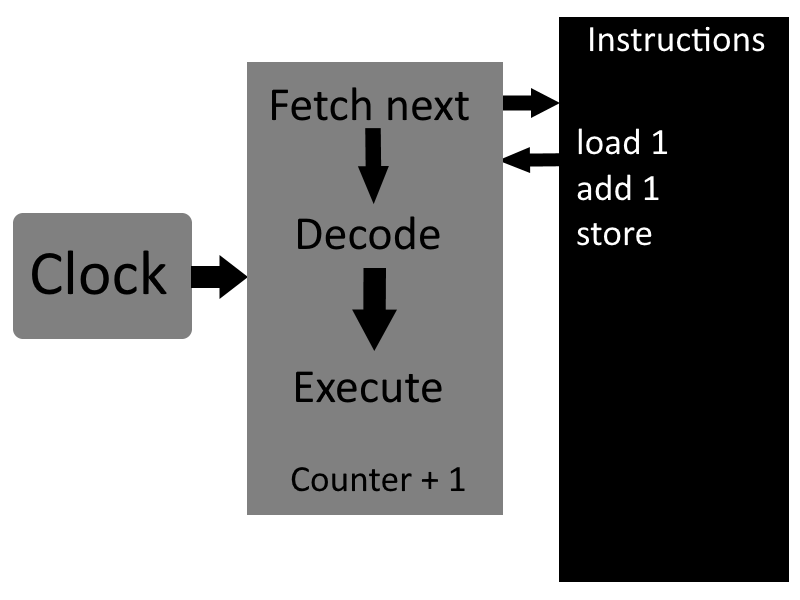
\includegraphics[scale=.4]{cpucycle.png}
\caption{CPU Cycle}
\end{figure}
\end{frame}

\begin{frame}{Linked Lists}
https://www.quick-bench.com/q/8GCHd74XnH1iguAkU8JmpRhgk9o
\end{frame}

\end{document}
